\section{Approach}
\label{sec:approach}
% \KZ{Also a general comment: be concise, and use pronouns where appropriate and not repeat things like Shiba Inu all the time. Also try not to use apostrophes after plurals, such as ``dogs' languages'' or ``audio samples' duration''. It's very rarely used these days.}%OK
 We now describe the method of constructing ShibaScript. To collect these clean Shiba Inu barks and endow them with corresponding transcripts, a six-step process is used.
 % \KZ{The overview pic must be more informative than
 % just a 6-step pipeline. Otherwise not much use.} The 6-step pic is omitted, I think it's redundant as we have pics in 2.1, 2.2, 2.3...
 These steps, in sequence, are  getting videos related to Shiba Inu dogs, extracting barks as ``sentences'' 
 %\KZ{on the granularity of seconds}, 
 removing barks with noise, extracting barks as ``words'', separating syllables, and clustering to assign appropriate phonemes based on their acoustic features.

 \subsection{Collecting Data}
 \label{sec:obtrainingshibainuvideos}
 %这里可以引用一些之前的works,那些works使用的数据集$
% \KZ{This section is a bit verbose. Avoid discussing routing engineering details
% and focus on the techinical challenges. Also the first para seems to repeat 
% things we already said in the intro. Don't repeat, but u can expand and 
% elaborate.}

% \KZ{Always include a tilde before cite like this: In former works ~\cite{ide2021rescue, ehsani2018let,molnar2008classification, hantke2018my}}
In this work, we aim at investigating the language patterns of Shiba Inu dogs. Previous works~\cite{ide2021rescue, ehsani2018let,molnar2008classification, hantke2018my} endeavor to understand dog language patterns conduct experiments on datasets~(\tabref{tab:previousdataset}) which have limited sizes and scenes.
% In former works~\cite{ide2021rescue, ehsani2018let,molnar2008classification, hantke2018my}, those who research on states of dogs have done experiments on datasets~(\tabref{tab:previousdataset}) which have limited sizes and scenes \MY{This sentence reads wordy. Rephrase as: Previous works endeavor to understand dog language patterns conduct experiments on .... }. 
Their frequent approach is to get several dogs and record their barks when dogs are put into the context of different events and in various kinds of places. The disadvantages of this method are three-fold. 
% \MY{Avoid saying anything is obvious unless it can be observed, just say that the disadvantages are three-fold}
First, the number of dogs is limited by the budget and practical conditions of these experiments. Second, such an approach can only include several ``typical scenarios'', and is almost impossible to cover all of the situations that dogs might experience in their daily lives. Third, field study like this is costly in terms of humans, machines, and time. Therefore it is hard to transfer the research to other animal species.
% \JY{say more}

\begin{table*}[th]
\centering
\small
\begin{tabular}{c|c|c|c|c|c}
\hline
\textbf{Name} & \textbf{Type} & \textbf{\# of Dogs} & \textbf{Scenes} & \textbf{Activities} & \textbf{Size} \\
\hline
Full Dataset~\cite{ide2021rescue}& video, audio, sensor & - & simulated disaster sites & - & 2825s \\
DECADE~\cite{ehsani2018let} & video, audio, sensor & 1 & indoors and outdoors & - & 4864s \\
Unknown~\cite{molnar2008classification} & audio & 14 & mostly indoors, street & - & 6,646 barks \\
EmoDog~\cite{hantke2018my} & audio & 12 & 7 fixed types & - & 9,447s \\
\textbf{ShibaScript} & audio, link & 16 & 37$\star$ & 44$\star$ & 14,702s$\star$ \\
\hline
\multicolumn{6}{l}{\small $\star$: The number of scenes and activities in ShibaScript is not fixed and can be expanded as the dataset is continuously collected. }
\end{tabular}

\caption{Dog-voice data sources used previously. 
Existing datasets are collected by manual recording. 
The first two contain videos of various lengths, 
while the latter two contain a certain amount of pure barks with pauses.}
% \KZ{There should be cites next to each Name. First is called ``Full Dataset''?
% 3rd row must have a name?! Why does the last column take up so much space?}}
\label{tab:previousdataset}
\end{table*}

%如果可以找得到YouTube数据量的话就更好了,引用一下,写完就去找
To solve these problems, we make use of the abundant resources from online social media. Each year, millions of videos are uploaded to YouTube, which is the largest video-sharing site around the world. These videos include large amounts of Shiba Inu dogs videos of different scenes uploaded by those who keep them. 
There are even people who set up an account specifically for dogs and upload hundreds or thousands of their videos. Collecting data from such Shiba Inu enthusiasts can substantially enlarge the number of dogs, cover more scenes, and reduce the cost. And most importantly, researchers can adapt this methodology to other dog breeds or even animal species, which means this approach is highly reusable.

We select 16 users who have uploaded plentiful Shiba Inu dogs videos and have relatively good recording conditions. These videos are the raw data.
% To protect their privacy, we anonimize user IDs. 
% The selection is based on several rules: (1) The videos are mainly about Shiba Inu dogs; (2) The user has 
% uploaded more than 400 videos (3) Videos were recorded under relatively good conditions. 

 \subsection{Extracting Sentences}
 \label{extractingsentences}
What we care and label transcripts for are the moments when dogs make any vocal expressions. Similar to humans, it is possible to define the sentence in the sound system of dog expressions. 
The definition is as below: In a sentence, dogs bark continuously on the granularity of seconds. Barks here represent the sounds dogs generate through vocal cord vibration.

In the videos we obtain from different YouTube users, there are a lot of irrelevant and silent frames when the concentrations of videos are not dogs or the dog in the current frame is not barking. 
% The points of the frames are not always Shiba Inu dogs. \MY{What is the points of the frames? Rephrase it.}
% Meanwhile, when the frames are focused on the dog, usually the dog is not barking. \MY{What's the purpose of this sentence?}

In order to extract the video clips containing vocal expressions of dogs.
% sentences dogs speak \MY{You haven't arrived at the stage where the structual is properly defined, here it is about sound event detection, avoid using ``dog speak'', just say extract video clips containing dogs vocal expressions}, which we define in the first paragraph. 
We use PANNs~\cite{kong2020panns}, a pretrained large sound event detection model including as many as 527 sound classes that can output audio tagging results as well as events’ on- and off- timestamps. Those frames which are tagged with ``bark'' in the top 10 results are considered to contain barks. We manually labeled 300 samples and compared them with PANNs output, a precision of 0.92 is observed.
%这里加一句统计数据
% \MY{What do you mean by saying quite well? You could say something like ``we manually labelled xx samples and compared with PANNs output, a precision of xx is observed.}

 \subsection{Removing Noises}
In constructing the dataset,  there is an apparent advantage of recording the audio of dogs in reality: the background noise and the conditions of the recording device can be better controlled. In this work, since we pursue better coverage of the dataset and 
use the resources from public social media, the problem of noises in the audio samples is inevitable. 

To generate the scripts and statistical results more accurately, we have tried our best to produce clean dog bark samples from two aspects: first in~\secref{sec:obtrainingshibainuvideos}, we have selected the users who uploaded videos with less noise and better recording conditions; 
and second, we use the following approach to significantly remove the noise from our data.
 
%这里可以增加一个噪音来源的文献
From artificial sampling, we find that the majority of the noises come from either the background music which the user edited into the video, or the human talking while the dog was barking. In order to remove this kind of noise, we make use of the result of PANNs as well. Those frames which are tagged with ``speech'' or ``music'' in the top 10 results are considered noisy frames. Sentences that contain noisy frames are filtered out. 

% and filter out the sentences detected of speech and music. 

% \KZ{Can you elaborate a bit on this (PANNs). 
% I think it's too simple for me to understand now. 

%There's also a thought that such
% noise removal method might subtantially reduce the number of sentence u have left.
% We need to counter such arguments.}(HOW HOW HOW).

 \subsection{Extracting Words}
 %插一个语言的词间隔时间的表格,需要查询资料

In the vocal expressions of dogs, there are mainly long pauses and short pauses. A long audio sample can be divided into several sentences with long pauses in between; a sentence can be further divided into several words with short pauses in between like in~\figref{fig:datasample}. We can define ``words'' in dogs statistically: In a word, dogs bark continuously on the granularity of microseconds.



% In human languages, each sentence contains multiple words. 
% A certain word in human languages represents an certain meaning. 
% Similarly, in dog ``language'', we can define words statistically: 
% In a word, dogs bark continuously on the granularity of microseconds. \KZ{A bark cannot be
% only a few microseconds, must be several tenths of a second.} 
% \KZ{Not sure what you are trying to say: We may not know whether words in a dog language represent any true meaning or not, 
% but there are possible differences among words and sentences because 
% there are different level length of pauses.} 
% An long audio sample can be divided into several sentences with long pauses in between; 
% a sentence can be further divided into several words with short pauses in between like in \figref{fig:datasample}.

\begin{figure}[th]
\centering
\scalebox{0.3}{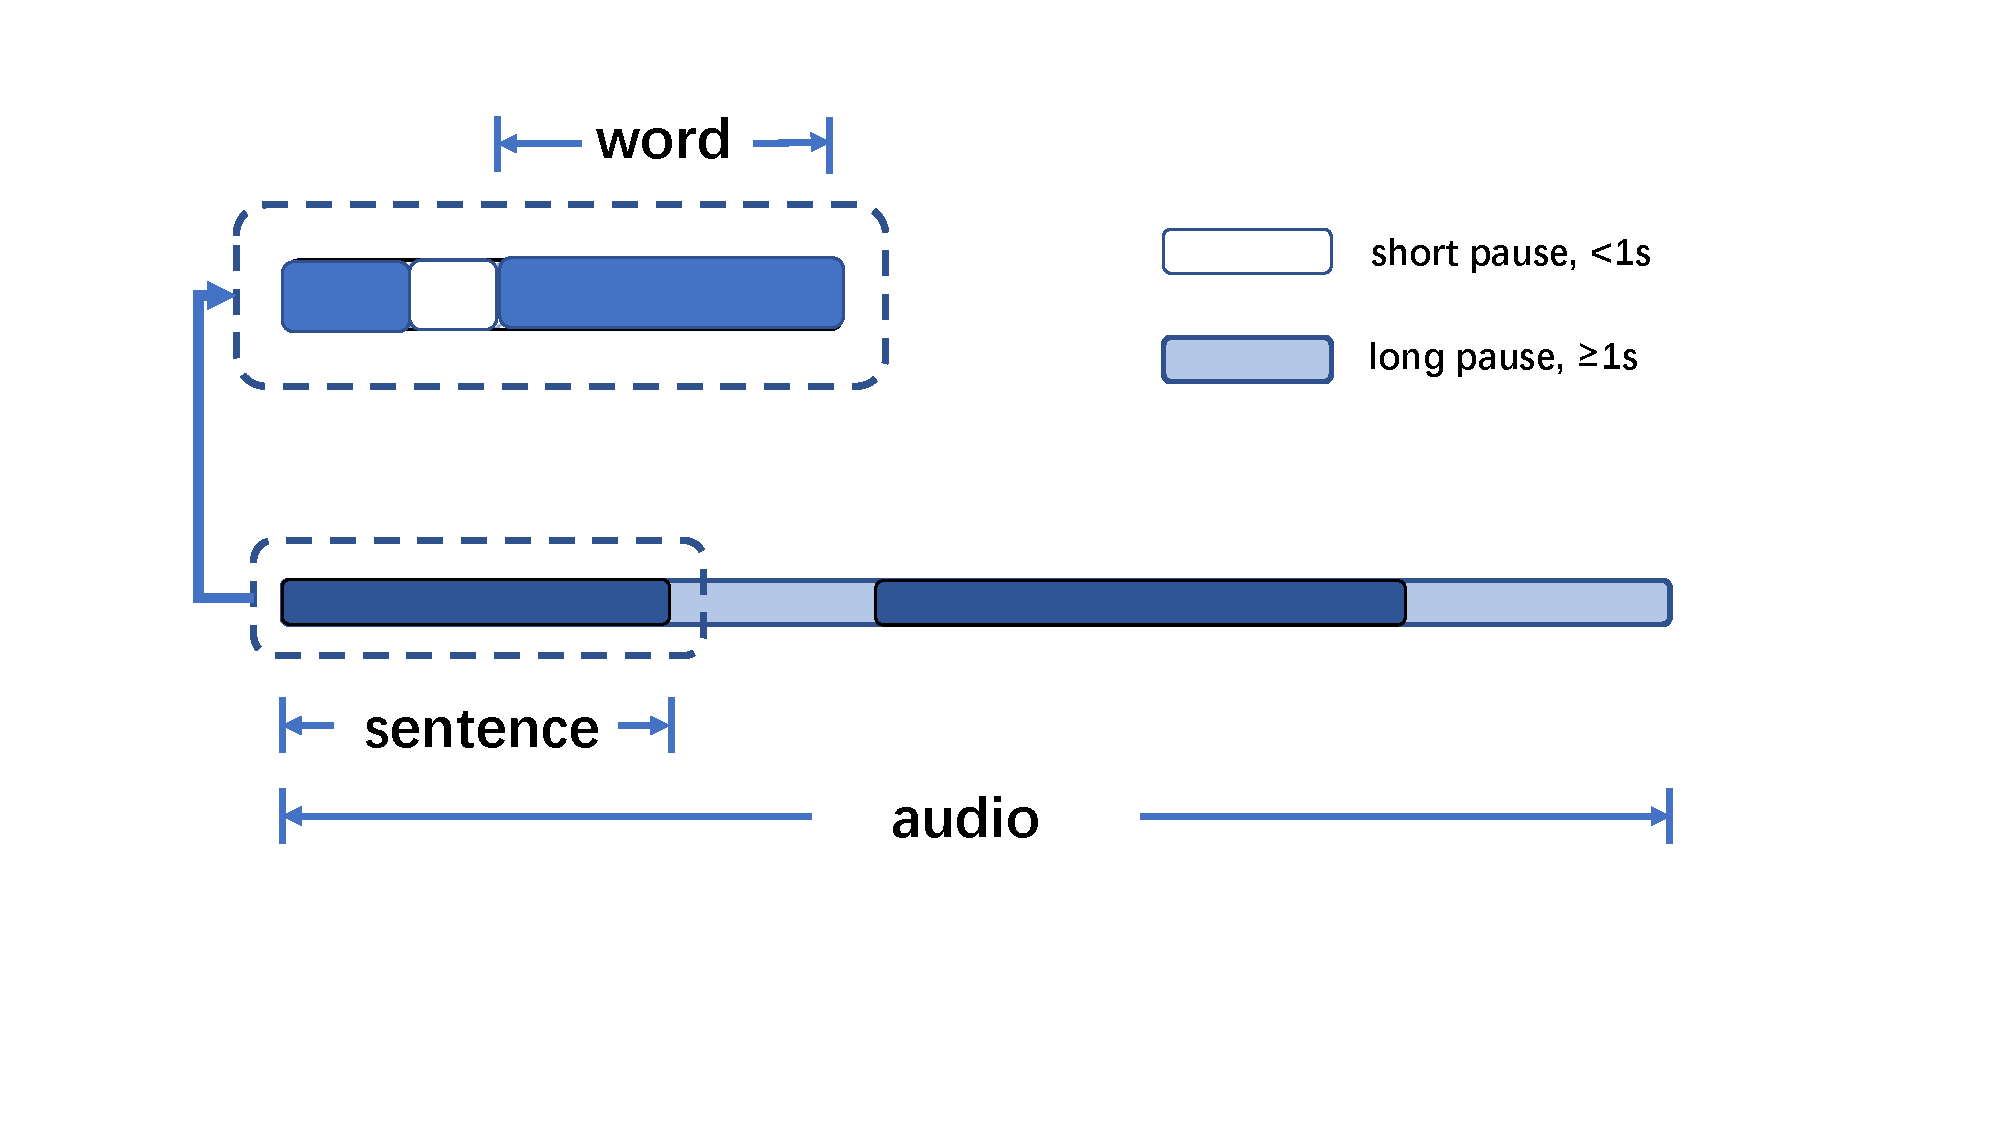
\includegraphics{sentence.pdf}}
\caption{The result of sentence-level and word-level split of a complete audio sample.}
\label{fig:datasample}
\end{figure}
% 模型与数据集
% \KZ{Use citet when you r using the citation as an
% entity: In \cite{hershey2021benefit}}

As mentioned in~\secref{extractingsentences}, the pre-trained model PANNs~\cite{kong2020panns} performed well on the task of sound event detection. 
%\KZ{You barely talked about PANNs.}
Besides the small-grid pauses, there may also be some noise that failed to be filtered in the previous step. To eliminate such small-grid pauses and noise, here we directly detect the ``barking'' event from the sentences, and do the word-level splitting based on it. In \citet{hershey2021benefit}, The authors picked out a subset of audios from the original AudioSet~\cite{gemmeke2017audio} and assigned ``strong'' labels to them(about 0.1 sec resolution). The strong-labeled subset of AudioSet results in improved model performance.

% 微调
We first trained a uniform model from PANNs for sound event detection on the strong-labeled subset of AudioSet. Then to extract words out of the sentence, we annotated strong labels on the event ``barking'', for 246 sentences with a total length of 715 seconds by the phonetic analysis tool Praat~\cite{boersma2001speak} and fine-tuned the pre-trained model. As shown in~\figref{fig:sed}, the finetuned model is used to detect the ``barking'' event and based on the onset and offset of the event, we can extract words from sentences and eliminate the short pauses.
% \KZ{If we define ``barking'' in its broadest sense, can PANNs barking class really
% include what we want?}
% \CH{The PANNs trained on AudioSet is not sufficient, the one finetuned on our dataset is sufficient}



\begin{figure}[th]
\centering
\scalebox{0.21}{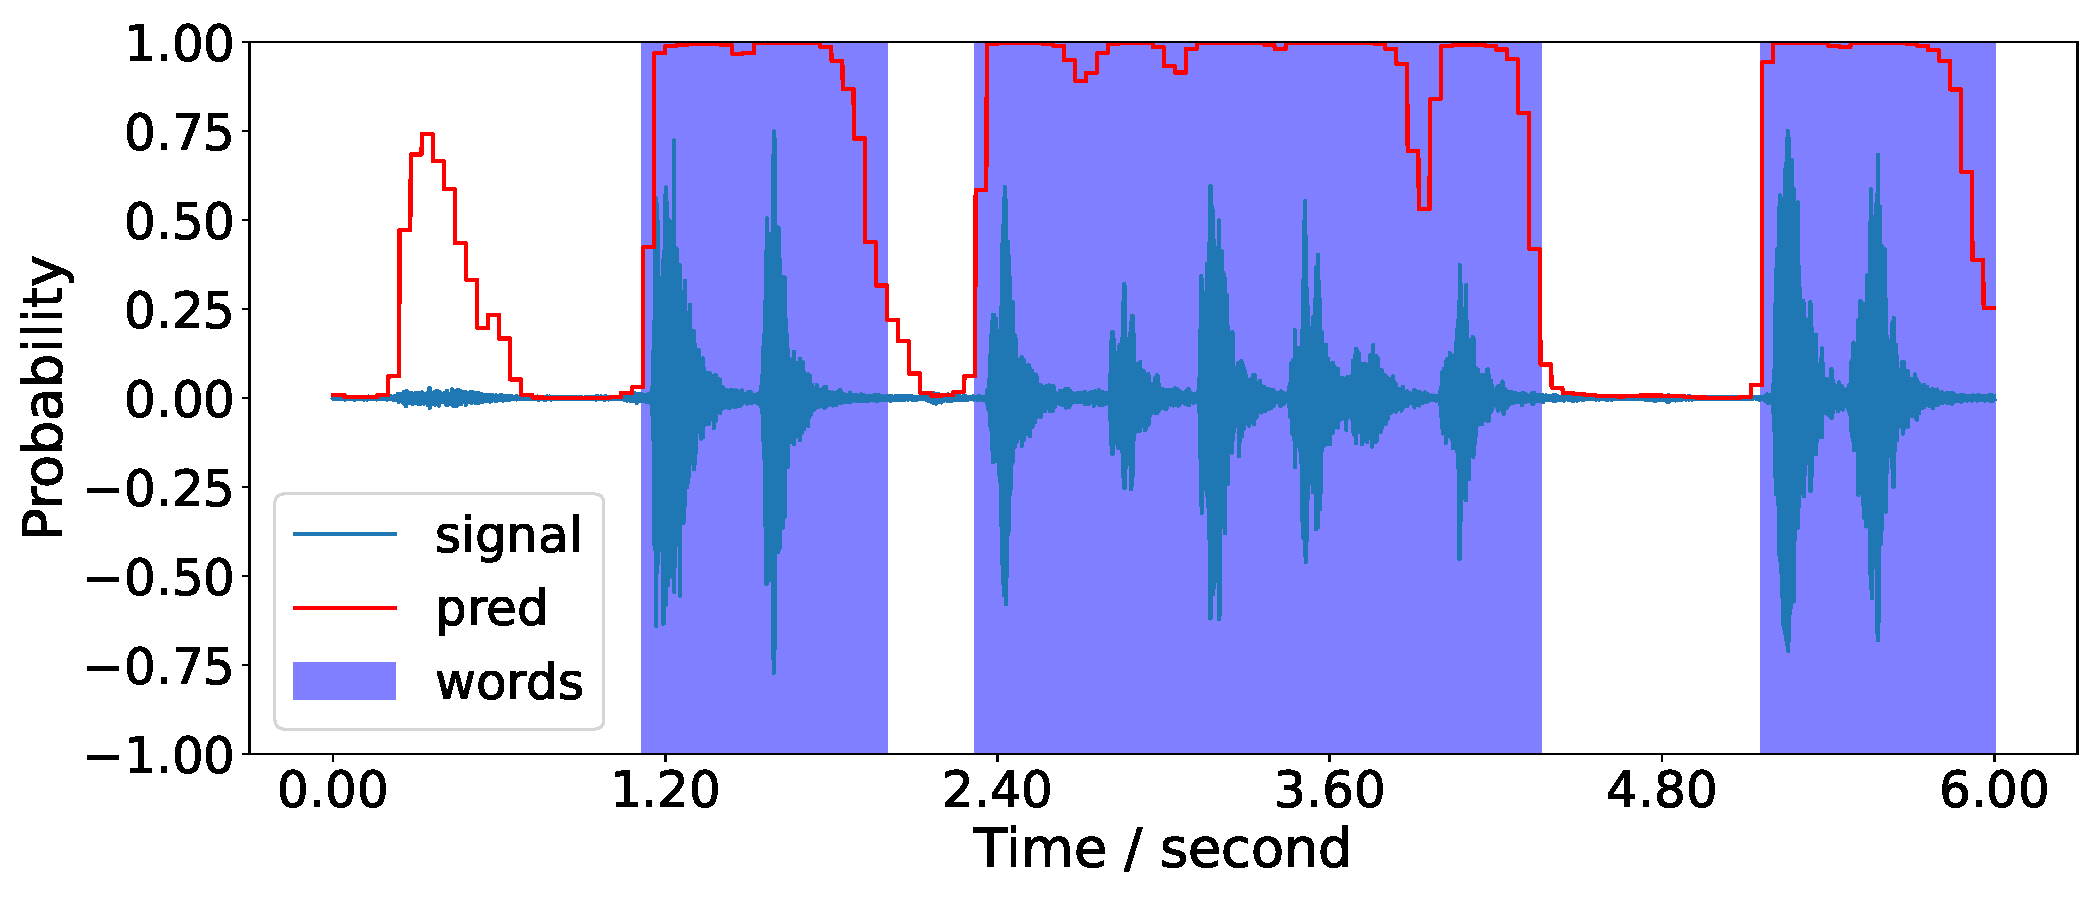
\includegraphics{sed.pdf}}
\caption{The SED model predicts whether the event ``barking'' existed in one frame. Words are extracted from the sentences by the onset and the offset.}
\label{fig:sed}
\end{figure}

%fine-tune the panns sound-event-detection model
%editted by chunhao

\subsection{Separating Syllables}
% \MY{A structure is needed here, that in human speech we have the minimum unit as phoneme that can construct syllables and words, based on which we form sentences with grammatical rules. We retain this setting in exploring dog language and define their barking sounds from the minimal unit, phonetic symbols. However, as dogs have different articulatory anatomy from humans, the sounds can be vastly different. We try to label dog sound excerpts with International Phonetic Alphabet.}

In human speech, we have the minimum unit as a phoneme that can construct syllables and words, based on which we form sentences with grammatical rules. We retain this setting in exploring dog language and define their barking sounds from the minimal unit, phonetic symbols~\cite{rohrmeier2015principles}. However, as dogs have different articulatory anatomy from humans, the sounds can be vastly different. We try to label dog sound excerpts with International Phonetic Alphabet (IPA).

% Syllables are the phonological \textit{building blocks} of words, 
% also the most natural phonetic component unit. 
% Take Internation Phonetic Alphabet~\cite{international1999handbook} as a reference, 
% it's comprehensive to transfer the concept of syllables to the barks of dogs. 

In \citet{rasanen2018pre}, the authors introduce that it is possible to do 
syllabification even when no priory linguistic knowledge exists. 
The way to segment speech into syllable-like units depends on sonority to 
show the edges of syllables~(\figref{fig:envelop}). Considering the fact that current 
dog voices are without any known language patterns, we can adopt this method to 
separate syllables in one word.

%这里插一张arthur的envelop图
\begin{figure*}[th]
\centering
\scalebox{0.40}{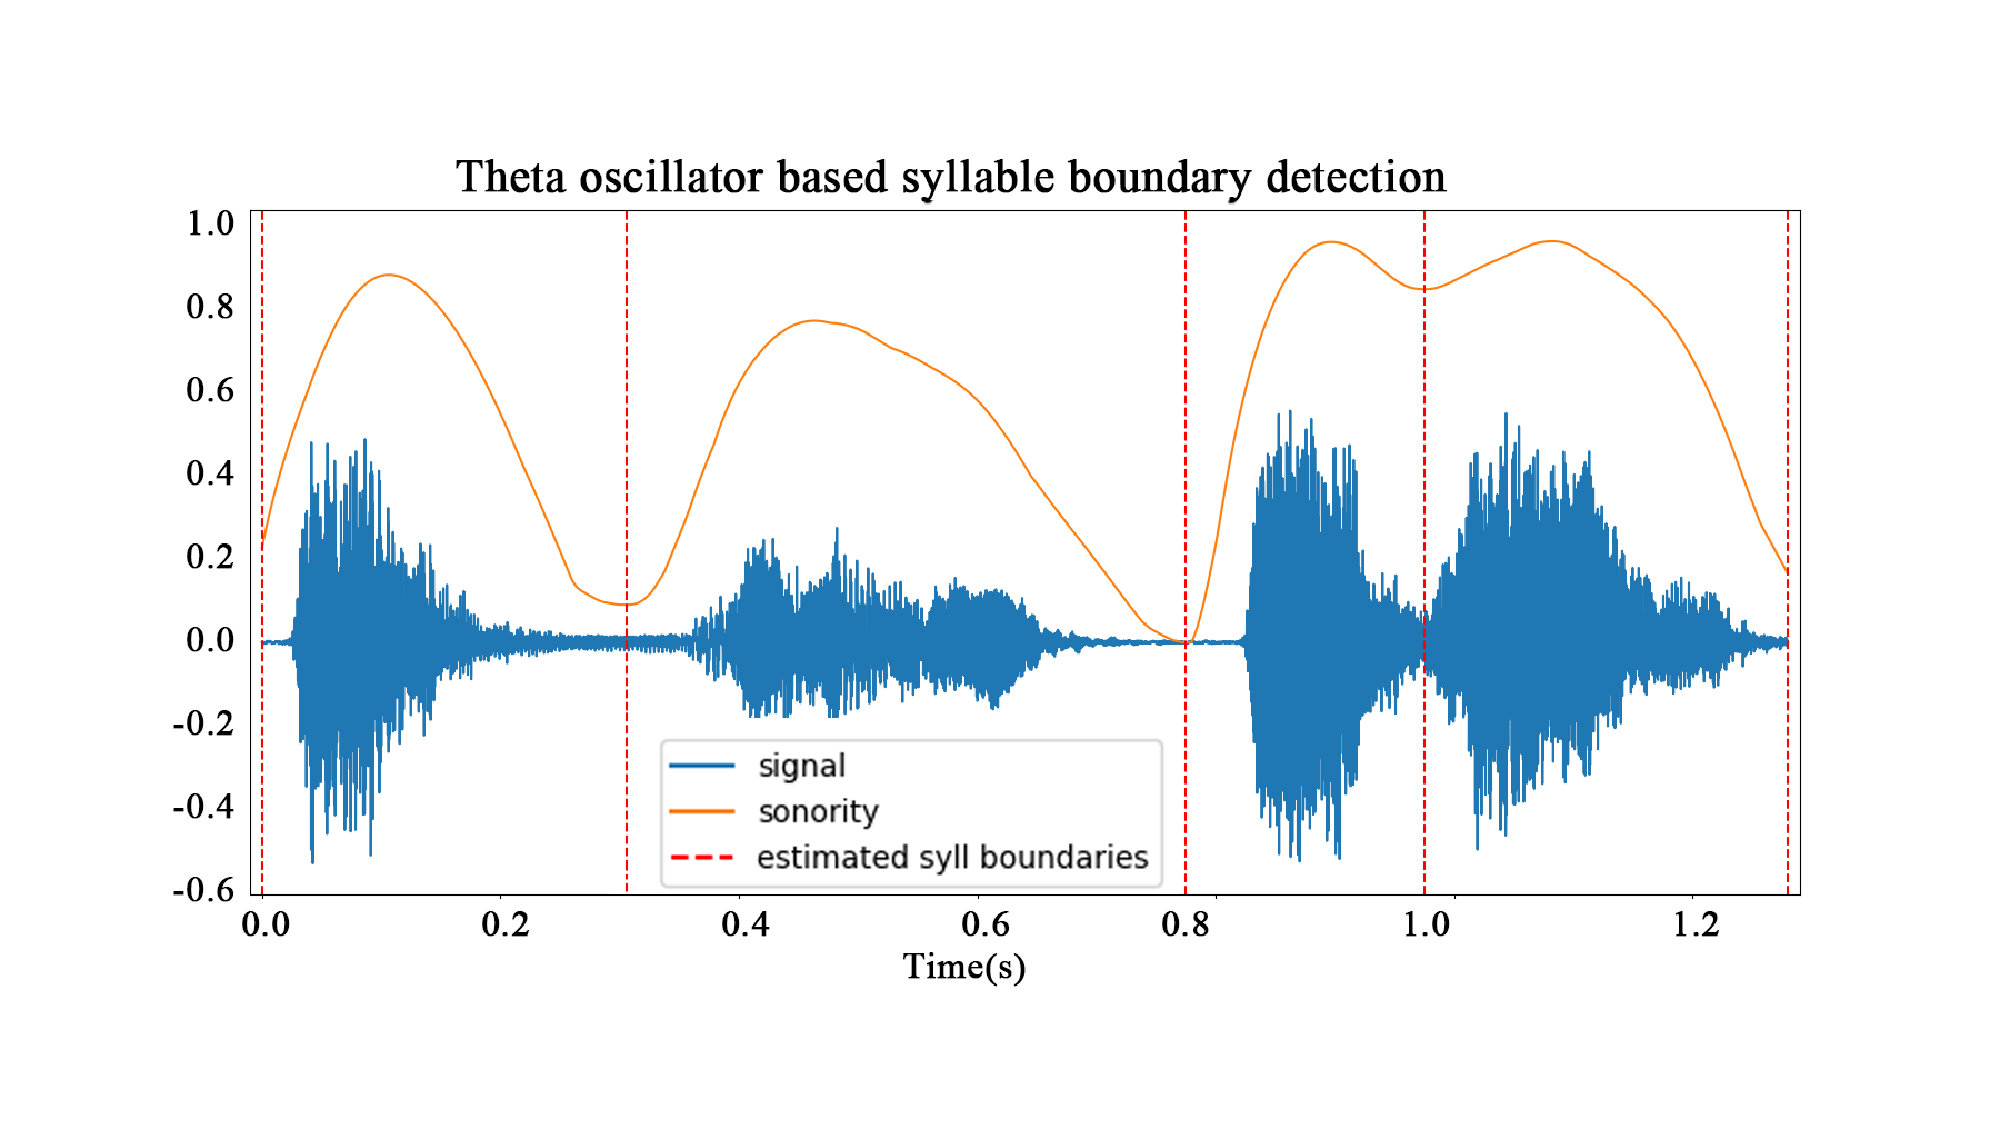
\includegraphics{boundary.pdf}}
\caption{Here a word is separated into four syllables based on the sonority. The complete transcript of this dog is shown in~\figref{fig:dataonesample}.}
\label{fig:envelop}
\end{figure*}

\subsection{Clustering and Phonemes Assignment}
\label{sec:clustering}

Given all these syllables and the assumption that dogs have a special system of syllables, 
we can do clustering and matching up to find a coexisting alphabet for Shiba Inu dogs. 
As these 16 dogs have different sex, ages, and physical conditions, 
we conduct Spectral Clustering~\cite{von2007tutorial} on syllables from 
one certain dog respectively. The feature we use is Filterbank~\cite{strang1996wavelets}. Generally, we set the number of clusters according to the number of videos of each dog, 
from 10 to 20 (the more videos, the more clusters). The clustering results after dimension reduction can be seen in~\figref{fig:visualizationcluster}:


%中插聚类可视化图片
% \begin{figure}[htbp]
% \centering
% \subfigure{
% \begin{minipage}[b]{.22\linewidth}
% \centering
% 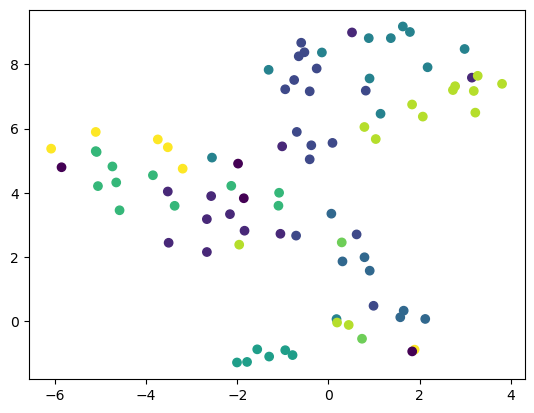
\includegraphics[scale=0.135]{cluster/shibainu_rikuchannel_sc.png}
% \end{minipage}
% }
% \subfigure{
% \begin{minipage}[b]{.22\linewidth}
% \centering
% 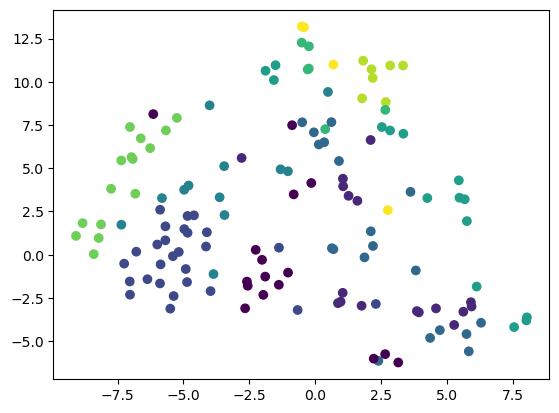
\includegraphics[scale=0.135]{cluster/ringoro_sc.png}
% \end{minipage}
% }
% \subfigure{
% \begin{minipage}[b]{.22\linewidth}
% \centering
% 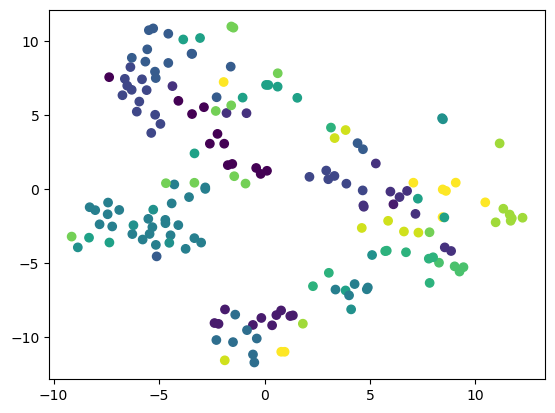
\includegraphics[scale=0.135]{cluster/hikaiti_sc.png}
% \end{minipage}
% }
% \subfigure{
% \begin{minipage}[b]{.22\linewidth}
% \centering
% 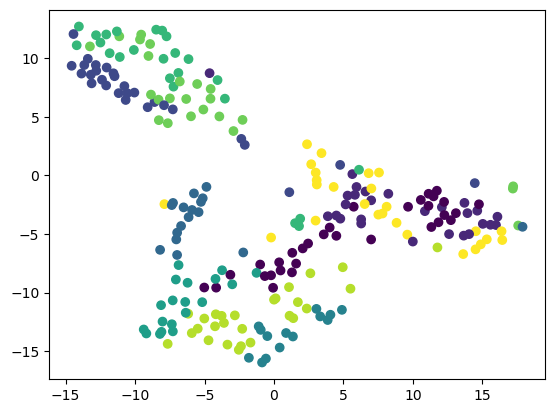
\includegraphics[scale=0.135]{cluster/jumpingmameko1822_sc.png}
% \end{minipage}




% \subfigure{
% \begin{minipage}[b]{.22\linewidth}
% \centering
% 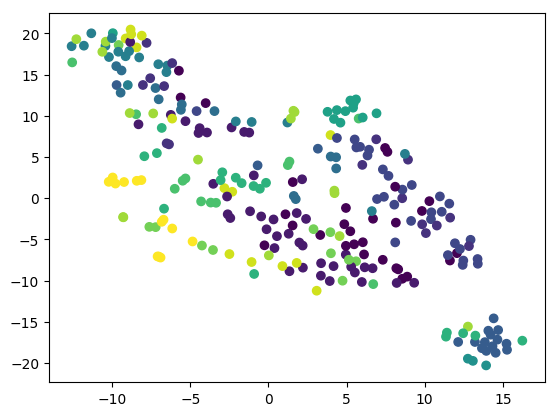
\includegraphics[scale=0.135]{cluster/shibaneko_sc.png}
% \end{minipage}
% }
% \subfigure{
% \begin{minipage}[b]{.22\linewidth}
% \centering
% 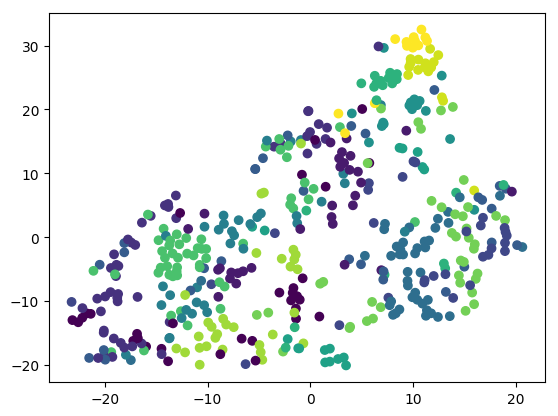
\includegraphics[scale=0.135]{cluster/shibainutakanoriawesomecha30_sc.png}
% \end{minipage}
% }
% \subfigure{
% \begin{minipage}[b]{.22\linewidth}
% \centering
% 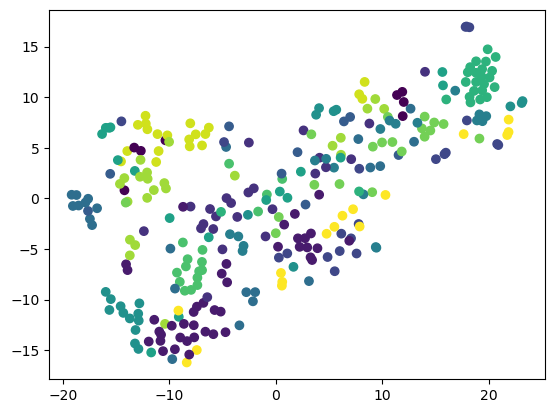
\includegraphics[scale=0.135]{cluster/MomoTenKuu_sc.png}
% \end{minipage}
% }
% \subfigure{
% \begin{minipage}[b]{.22\linewidth}
% \centering
% 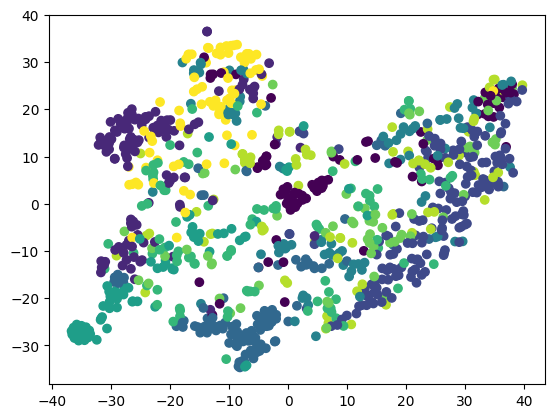
\includegraphics[scale=0.135]{cluster/mamedachamesuke_sc.png}
% \end{minipage}


\begin{figure}[th]
\centering
\scalebox{0.45}{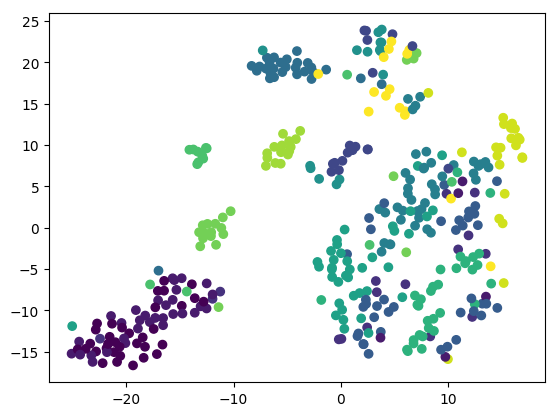
\includegraphics{cluster/ShibainuRanmaru_sc.png}}
\caption{2-D Visualization of spectral clustering of one dog's data using t-SNE. 
The complete clustering of all dogs can be checked in~\secref{sec:appendixb}.}
\label{fig:visualizationcluster}
\end{figure}


% \subfigure{
% \begin{minipage}[b]{.22\linewidth}
% \centering
% 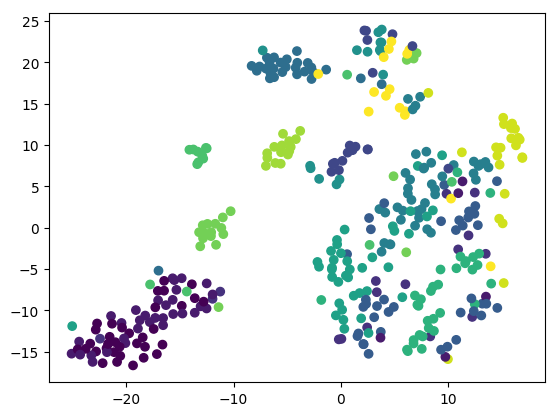
\includegraphics[scale=0.135]{cluster/ShibainuRanmaru_sc.png}
% \end{minipage}
% }
% \subfigure{
% \begin{minipage}[b]{.22\linewidth}
% \centering
% 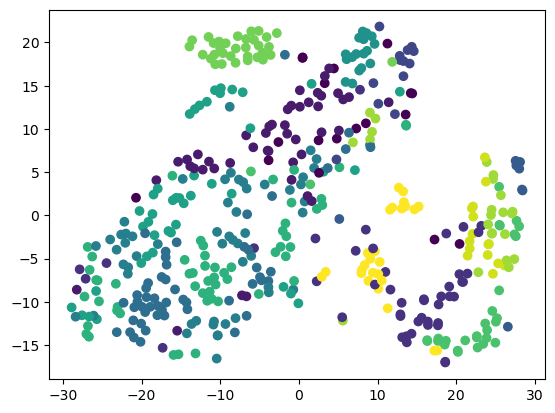
\includegraphics[scale=0.135]{cluster/shibainu-rara_sc.png}
% \end{minipage}
% }
% \subfigure{
% \begin{minipage}[b]{.22\linewidth}
% \centering
% 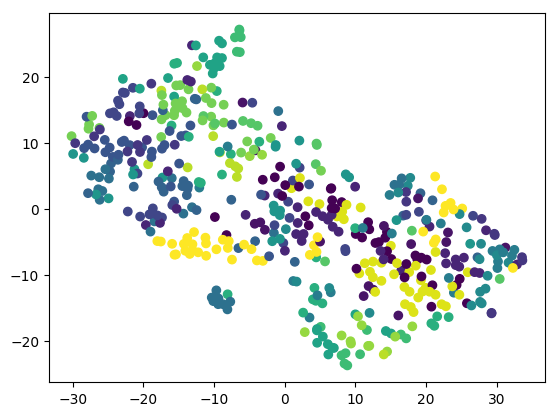
\includegraphics[scale=0.135]{cluster/ShibainuKOTETSU_sc.png}
% \end{minipage}
% }
% \subfigure{
% \begin{minipage}[b]{.22\linewidth}
% \centering
% 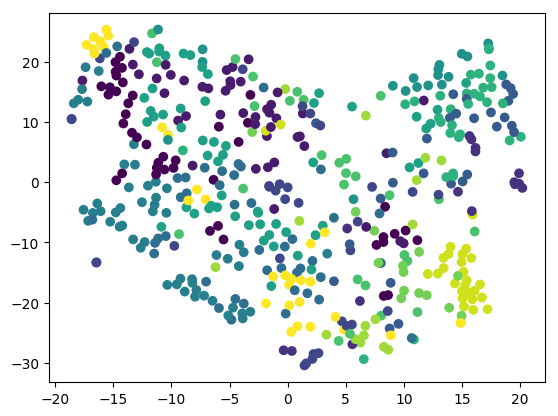
\includegraphics[scale=0.135]{cluster/shibainucatchannel7691_sc.png}
% \end{minipage}
% }


% \subfigure{
% \begin{minipage}[b]{.22\linewidth}
% \centering
% 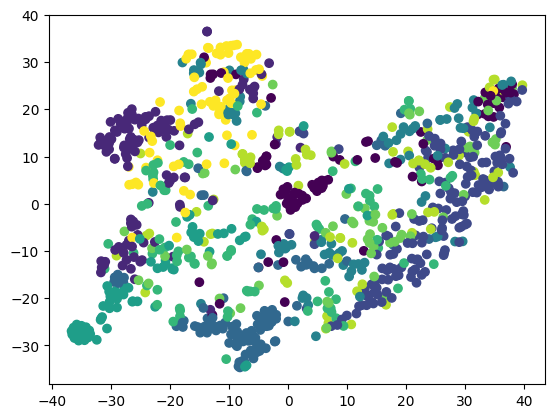
\includegraphics[scale=0.135]{cluster/mamedachamesuke_sc.png}
% \end{minipage}
% }
% \subfigure{
% \begin{minipage}[b]{.22\linewidth}
% \centering
% 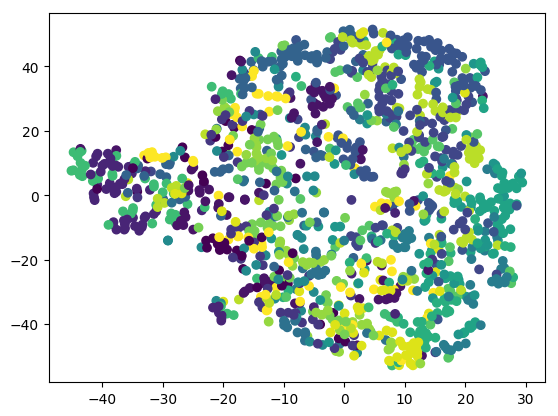
\includegraphics[scale=0.135]{cluster/user-kd8rn5jx7x_sc.png}
% \end{minipage}
% }
% \subfigure{
% \begin{minipage}[b]{.22\linewidth}
% \centering
% 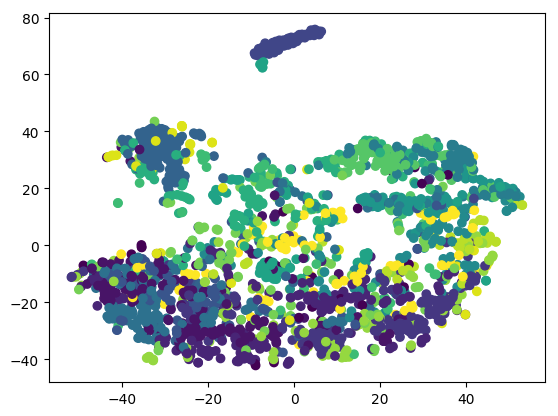
\includegraphics[scale=0.135]{cluster/shibainuTAIGA_sc.png}
% \end{minipage}
% }
% \subfigure{
% \begin{minipage}[b]{.22\linewidth}
% \centering
% 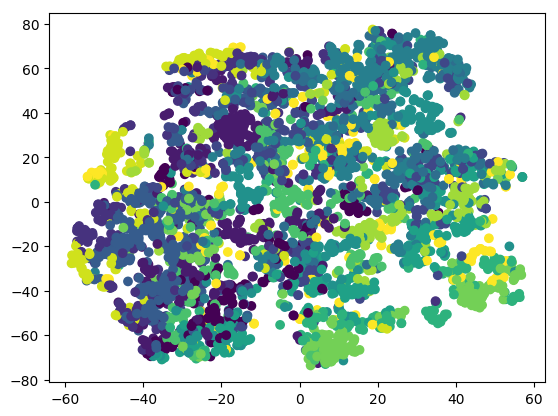
\includegraphics[scale=0.135]{cluster/ShibaInuKohachannel.png}
% \end{minipage}



% }



% \caption{Visualization of Spectral Clustering after TSNE. The dog's IDs are increasing from left to right, up to down. \KZ{If there's no enough space, you can show one or two pics here and include the rest in the appendix.}}
% \label{fig:visualizationcluster}
% \end{figure}




After clustering, we have found that compared to human languages, dogs have fewer phonetic categories, which is understandable because humans have a more complex vocal system. Aggregating all the clustering results together, we refer to IPA for illustration and find nine consistent syllables~(\tabref{tab:alphabet}). After setting up the syllables dictionary, we can reversely get the words transcripts with short pauses, sentences transcripts with long pauses and audios transcripts with pauses.

% a
% ^
% i
% u
% u:
% k
% en
% au
% (w)au
\begin{table}[th]
\centering
\small
\begin{tabular}{l|l}
\hline
\textbf{Symbol} & \textbf{Description}\\
\hline
\verb|[a]| & \href{https://drive.google.com/file/d/1tobgLGw4VmCyT5DgltnAGF99hI0-isiv/view?usp=share_link}{Steady pronunciation} \\
\verb|[^]| & \href{https://drive.google.com/file/d/1QvvKeNjLhHYxpa9ehePRCO2AlzDZrouU/view?usp=share_link}{Contains strong sounds}\\
\verb|[i]| & \href{https://drive.google.com/file/d/1C5Y5-a7oEKNWcwy03MRf1UooOaHxpJJ2/view?usp=share_link}{Stridulation}\\
\verb|[u]| & \href{https://drive.google.com/file/d/1NzEY9oxAvNy8H_Jo5qEOIzYwOIAafOGw/view?usp=share_link}{Lasts for short}\\
\verb|[u:]| & \href{https://drive.google.com/file/d/15uOnxgU1k4TGZmgQrOQ0Btb8FttHMNEi/view?usp=share_link}{Lasts for long}\\
\verb|[k]| & \href{https://drive.google.com/file/d/1568I7KdnbtLDueXXBnBKU5yCseLgQAY4/view?usp=share_link}{Sounds like knocking}\\
\verb|[en]| & \href{https://drive.google.com/file/d/1R7wEkBSzxPS_6YaNG0z4YGB_9VmjqPzt/view?usp=share_link}{Sounds like [ng] in English}\\
\verb|[au]| &  \href{https://drive.google.com/file/d/1ZhJWxb24QBpgdzdN_-TIbc4_ma3TCsmS/view?usp=share_link}{Ends with sounds like [o]} \\
\verb|[(w)au]| & \href{https://drive.google.com/file/d/1vJ10GUSh2XSF3cyNvQAQuHyrtrWzU31t/view?usp=share_link}{Starts with [w]} \\

\hline
\end{tabular}
\caption{The nine types of syllables as well as the syllables description of Shiba Inu. 
Every description is a clickable hyperlink to an actual sound sample.}
\label{tab:alphabet}
\end{table}

A typical symbolic transcript of one audio sentence can be in~\figref{fig:dataonesample}.

% \begin{table}[]
%     \centering
%     \begin{tabular}{c|c}
%          &  \\
%          & 
%     \end{tabular}
%     \caption{Caption}
%     \label{tab:my_label}
% \end{table}

% %这里插一个典型的图
% \begin{table}[th]
% \small
% \begin{center}
% \begin{tabular}{ l l l }
% \hline
%  \verb|sentence_id| & \verb|200_1| &  \\ 
%  \verb|from_video| & \verb|video200| &  \\  
%  \verb|sentence_start_time| & \verb|25| & \\    
%  \verb|sentence_end_time| & \verb|27| & \\
%  \verb|words_info| & \verb|word_id| & \verb|200_1_0| \\
%   & \verb|from_sentence| & \verb|200_1| \\
%   & \verb|word_start_time| & \verb|25.56| \\
%   & \verb|word_end_time| & \verb|25.92| \\
%   & \verb|transcript| & \verb|a| \\
%   & \verb|syllables| & \verb|0.0, 0.36| \\
%   & \verb|word_id| & \verb|200_1_1|\\
%   & \verb|from_sentence| & \verb|200_1| \\
%   & \verb|word_start_time| & \verb|26.2| \\
%   & \verb|word_end_time| & \verb|26.32|\\
%   & \verb|transcript| & \verb|a|\\
%   & \verb|syllables| & \verb|0.0, 0.12|\\
% \verb|transcript| & \verb|a; a| & \\
% \hline
% \end{tabular} 
% \end{center}
% \caption{A script of one sentence, containing the id of this sentence, the source audio id, the time of this sentence in the audio, the words and their information in this sentence.
% \KZ{This example is not so effective. It doesn't look like a symbol script to me cos it only has a; a. Can u make it more interesting? Do not use an image as a table here. Draw the table properly in LaTeX.}}
% \label{tab: datasetonesample}
% \end{table}

\begin{figure}[th]
\centering
\scalebox{0.35}{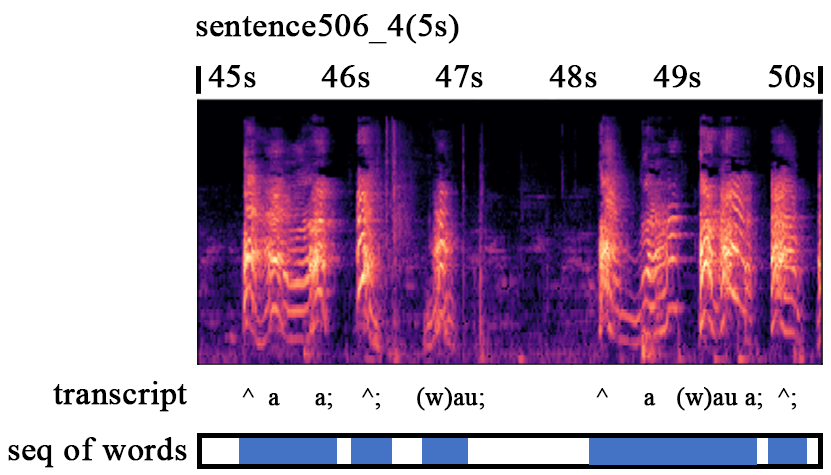
\includegraphics{dataonesample.png}}
\caption{The script of the sentence in the introduction, containing the id of this sentence, the source audio id, the time of this sentence in the audio, the 5 words and their information in this sentence. Each word in the ``transcript'' is splitted by ``;''.}
% \KZ{Didn't u use ; to separate the words within a sentence in a transcript? In the fig, it should be ``seq of words'' instead of ``word''? There's multiple words in a sentence. The coloring and style of the bar for ``words'' should be
%  the same as  Fig. 2. Now the coloring is not consistent.}
\label{fig:dataonesample}
\end{figure}

